\problemname{That's One Hanoi-ed Teacher}

Roberta Roberts (the older sister of Bobby in Problem F) teaches math at a small
college, and has just introduced the Tower of Hanoi to the students in her
Discrete Math class. In case you've been in a Tibetan monastery for the past
several years and have never heard of the Tower of Hanoi puzzle (doubtful for
several reasons), here's a brief description. The puzzle consists of three pegs,
and $n$ disks with radii of $1, 2, \ldots, n$.  The initial set up has all the
disks on a {\em start\/} peg in increasing order of their size from top to bottom,
forming a pyramid.  The object of the puzzle is to move all of these disks to
a {\em destination\/} peg using the following rules:
\begin{enumerate}
\item You can move only one disk at a time
\item At no point may a larger disk lie on top of a smaller disk
\end{enumerate}
It's well known that the optimal (i.e., shortest) solution for a Tower of Hanoi
puzzle with $n$ disks involves $2^n-1$ moves.  The optimal
solution for $n=3$ is shown below (where the start peg is the leftmost peg and
the destination peg is the rightmost peg):
\begin{center}
\scalebox{0.8}{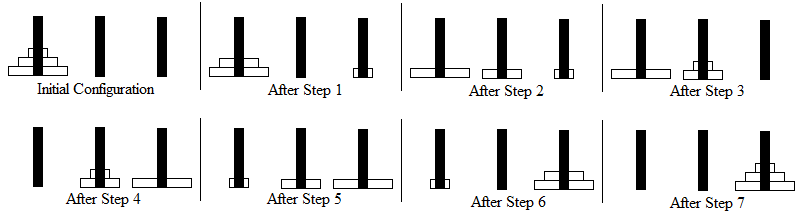
\includegraphics{hanoi2}}\\
Figure G.1
\end{center}
As part of an in-class lab, Roberta will hand out Tower of Hanoi sets to her students and let them try to solve the problem on their own.  As she goes around the room, she realizes that for the larger size sets, she has trouble looking at a current layout of the disks and determining whether the student is on the right track or not.
In other words, she wishes to know whether or not a given configuration of the puzzle is one of the $2^n$ configurations in the optimal solution sequence. She would also like to
be able to tell her students how close they are to the final configuration (i.e., all
the disks in increasing sizes, top to bottom, on the destination peg).
Needless to say, this has caused her a bit of consternation, so she has come to you for help.

\section*{Input}
Input consists of three lines, each line representing one peg of a Tower of Hanoi configuration.
Each of these lines starts with a non-negative integer $m$ indicating the number
of disks on that peg, followed by $m$ integers indicating the disks, starting
with the disk on the bottom of the peg.  The first line 
refers to the start peg and the last line refers to the destination peg.
Disks are numbered consecutively starting at 1 with each number indicating the\
disk's radius.  All disk numbers used form a consecutive sequence. The
maximum number of disks in any test case is 50.

\section*{Output}
Display {\tt No} if the given configuration is not in the optimal solution sequence; otherwise display the minimum number of remaining moves required to get to
the final configuration.

\pagebreak


